
%
%\begin{frame}[fragile, c]{Message flow}
%
%%TODO: Vllt auf "Standardfall" wie im Programm einschränken
%\lstset{
%	style=default,
%	frame=none
%}
%\begin{figure}[H]
%\centering
%\begin{lstlisting}
%§\textbf{Client}§                                       §\textbf{Server}§
%
%ClientHello        -------->
%                                      ServerHello
%                               ServerCertificate*
%                               ServerKeyExchange*
%                   <--------      ServerHelloDone          
%ClientKeyExchange
%[ChangeCipherSpec]
%Finished           -------->
%                               [ChangeCipherSpec]
%                   <--------             Finished
%[Application Data] <------->   [Application Data]
%\end{lstlisting}
%\end{figure}
%
%\begin{flushright}
%\tiny \textit{Based on the TLS 1.2 specification, RFC 5246.}
%\end{flushright}
%
%\end{frame}

%\begin{frame}[c]{Cipher suites}
%\centering
%TLS\_{\color{svshellblau2}RSA}\_WITH\_{\color{svsrot}AES\_128\_CBC}\_{\color{svsgrau2}SHA}
%
%\vspace{1cm}
%
%TLS\_{\color{svshellblau2}DHE\_RSA}\_WITH\_{\color{svsrot}AES\_128\_GCM}\_{\color{svsgrau2}SHA256}
%\end{frame}








% Original
% --------------------------------------

\section{Der Arbeitsbereich SVS} % erscheint in Agenda
\subsection{Mission} % erscheint in Agenda
\subsection{Themen} % erscheint in Agenda
\subsection{Kontakt} % erscheint in Agenda

\begin{frame}
	\frametitle{Der Arbeitsbereich Sicherheit in Verteilten Systemen (SVS)}
	\begin{block}{Lorem ipsum dolor}
		Lorem ipsum dolor sit amet, consectetur adipisicing elit, sed do eiusmod tempor incididunt ut labore et dolore magna aliqua. Ut enim ad minim veniam, quis nostrud exercitation ullamco laboris nisi ut aliquip ex ea commodo consequat. 
	\end{block}
	\begin{itemize}
		\item Themen
			\begin{enumerate}
				\item Privacy Enhancing Technologies (PET)
				\item Security Management \& Risk Management
				\item Security of Mobile Systems
			\end{enumerate}
		\item Weitere Informationen
			\begin{itemize}
				\item http://www.informatik.uni-hamburg.de/svs
			\end{itemize}
	\end{itemize}
\end{frame}

\section{Beispiel für eine Abbildung} % erscheint in Agenda

\subsection{Zugangskontrolle} % erscheint in Agenda
\begin{frame}
	\frametitle{Beispiel für eine Abbildung}
	\begin{itemize}
		\item Zweck
			\begin{itemize}
				\item Nur mit \alert{berechtigten Partnern} weiter kommunizieren
				\item Verhindert unbefugte Inanspruchnahme von Betriebsmitteln
			\end{itemize}
	\end{itemize}
	\vspace{\fill}
	\pause % Das Nachfolgende erst nach Klick einblenden...
	\begin{center}
		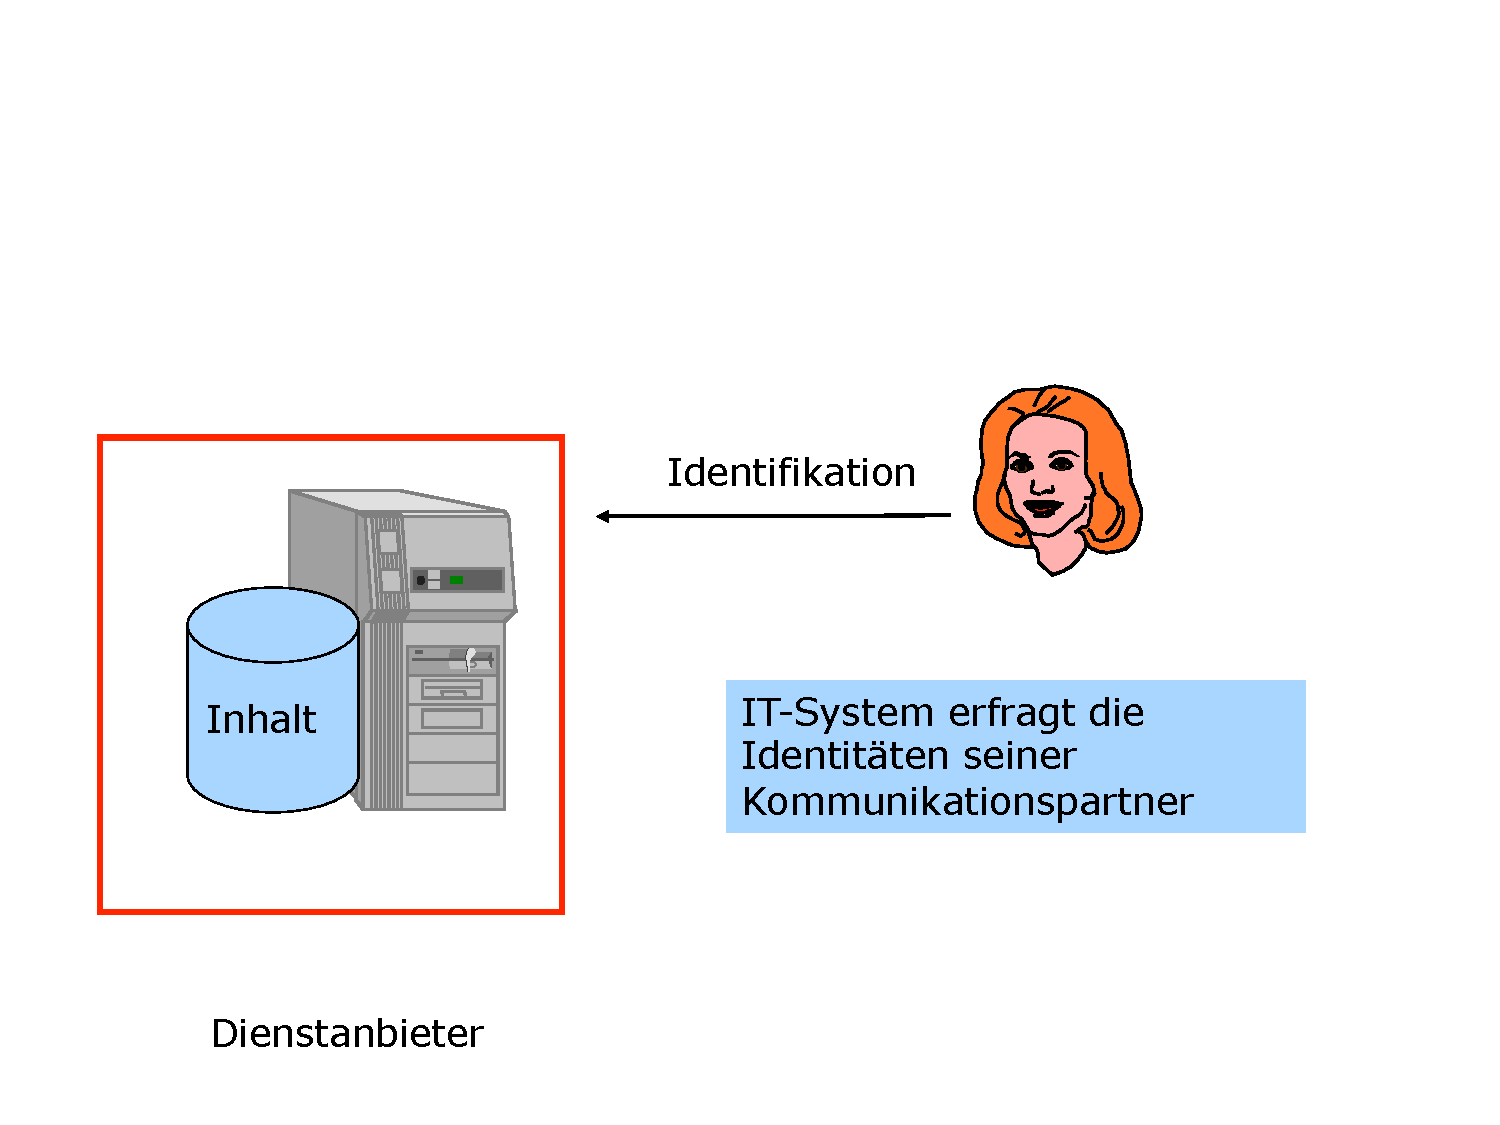
\includegraphics[width=0.8\textwidth]{pic/abbildung1.pdf}
	\end{center}
\end{frame}

\subsection{DRM-Systeme} % erscheint in Agenda

\begin{frame}
	\transwipe % funktioniert nur bei Anzeige mit Acrobat Reader
	\frametitle{Beispiel für eine Abbildung}
	\begin{itemize}
		\item Zweck
			\begin{itemize}
				\item Einem Kunden \emph{\color[RGB]{0,128,0} K} einen Inhalt \emph{\color{red} I} in einer bestimmten Weise zugänglich machen, ihn aber daran hindern, \emph{alles} damit tun zu können.
			\end{itemize}
	\end{itemize}
	\vspace{\fill}
	\begin{center}
		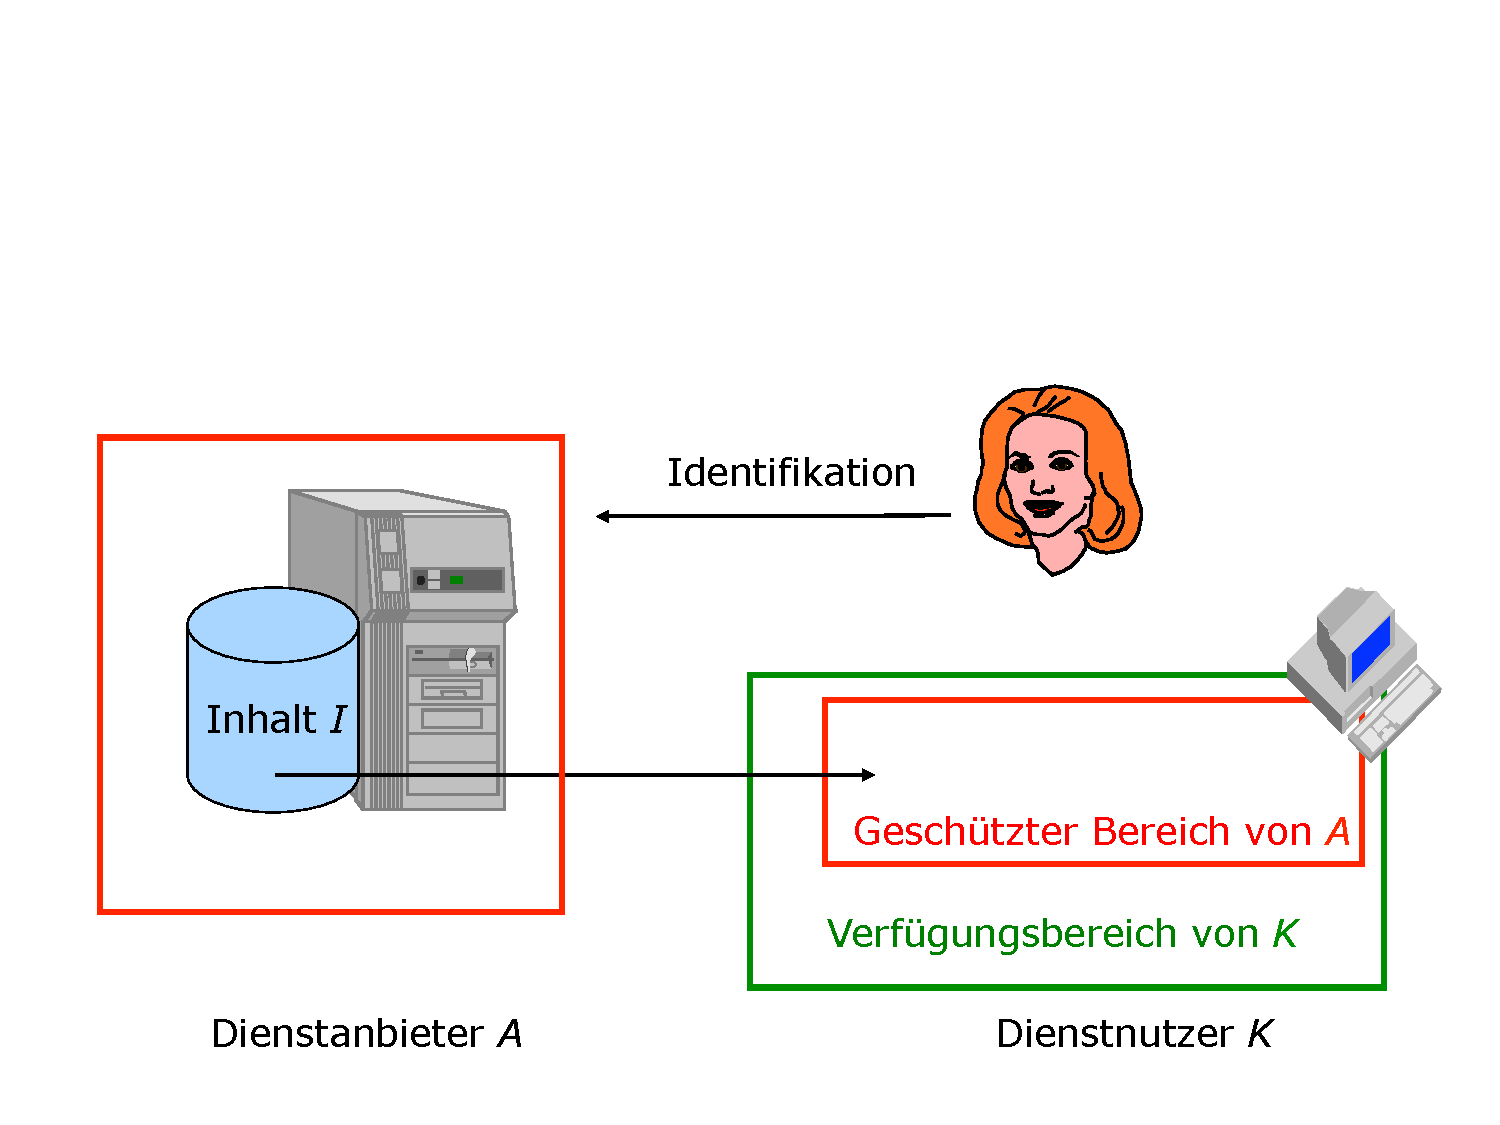
\includegraphics[width=0.8\textwidth]{pic/abbildung2.pdf}
	\end{center}
\end{frame}

\section{Weiteres Beispiel für eine Abbildung} % erscheint in Agenda

\begin{frame}
	\frametitle{Weiteres Beispiel für eine Abbildung}
	\framesubtitle{[John Doe, 1966] }
	\begin{itemize}
		\item Voraussetzung: {\color{black} Angreifer} 
			\begin{itemize}
				\item betreibt täuschend echte Webseite der Bank
				\item bewegt den Kunden zum Besuch dieser Seite
			\end{itemize}
	\end{itemize}
	\vspace{\fill}
	\begin{center}
		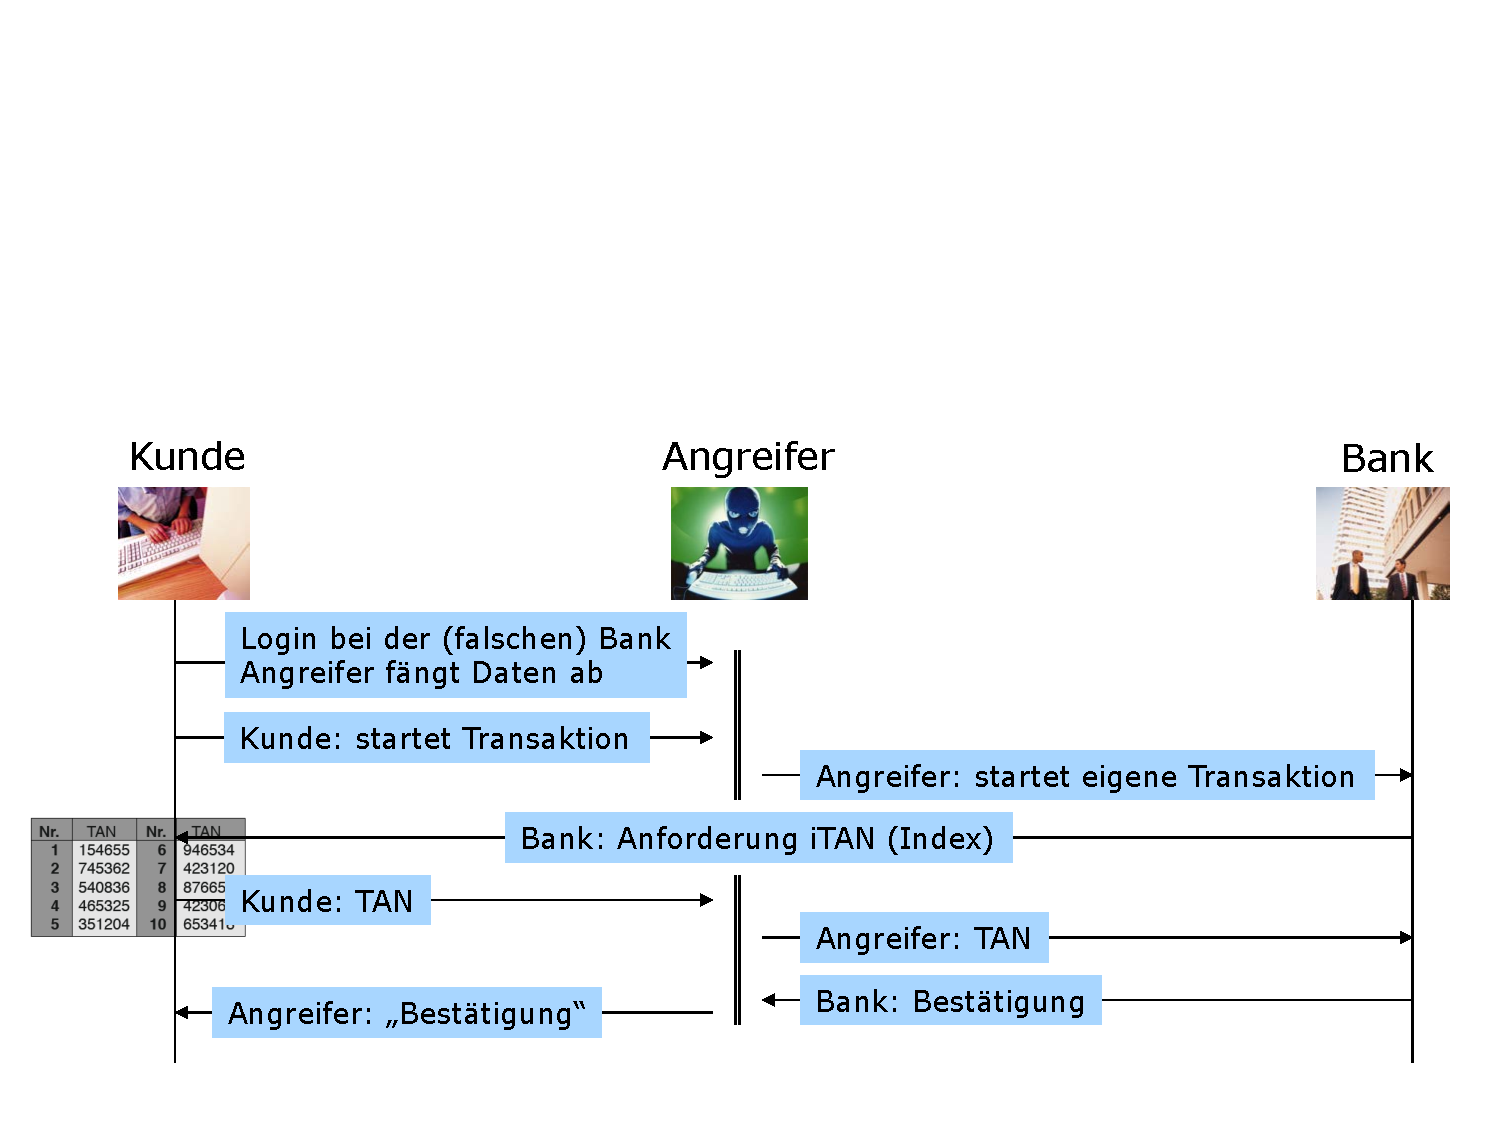
\includegraphics[width=\textwidth]{pic/abbildung3.pdf}
	\end{center}
\end{frame}

\section{Ebenen} % erscheint in Agenda

\begin{frame}
	\frametitle{Ebenen}
	\begin{itemize}
		\item Erste Ebene
			\begin{itemize}
				\item Zweite Ebene
				\begin{itemize}
					\item Dritte Ebene
				\end{itemize}
				\item Zweite Ebene
			\end{itemize}
		\item Erste Ebene
	\end{itemize}
	\begin{enumerate}	
		\item Erste Ebene
			\begin{enumerate}
				\item Zweite Ebene
				\begin{enumerate}
					\item Dritte Ebene
				\end{enumerate}
				\item Zweite Ebene
			\end{enumerate}
		\item Erste Ebene
	\end{enumerate}
\end{frame}

\section{Spalten} % erscheint in Agenda

\begin{frame}{Spalten}
	\begin{columns}[T]
		\begin{column}{.6\textwidth}
			\begin{itemize}
				\item Linke Spalte
				\begin{itemize}
					\item Lorem ipsum dolor sit amet, 
					\item consectetur adipisicing elit, 
					\item sed do eiusmod tempor incididunt ut 
					\item labore et dolore magna aliqua. 
				\end{itemize}
				\item Erste Ebene
				\begin{itemize}
					\item Zweite Ebene
					\item Zweite Ebene
				\end{itemize}
				\item Erste Ebene
				\begin{itemize}
					\item Zweite Ebene
					\item Zweite Ebene
				\end{itemize}
			\end{itemize}
		\end{column}		
		\begin{column}{.4\textwidth}
			\begin{center}
				\vspace{1cm}
				
\includegraphics[width=2.2cm]{pic/svs_logo_hires-ohne-was.png} \\
				Das SVS-Logo				
			\end{center}
		\end{column}
	\end{columns}	
\end{frame}